\documentclass{standalone}

\usepackage{amsmath}
\usepackage{tikz}
\usetikzlibrary{arrows.meta, positioning, calc}

% Respect chosen fonts (serif) and metrics
\renewcommand{\familydefault}{\rmdefault}

%% font
\usepackage{dsfont}
\usepackage[T1]{fontenc}
\usepackage{lmodern}
\usepackage{amsmath}

\begin{document}

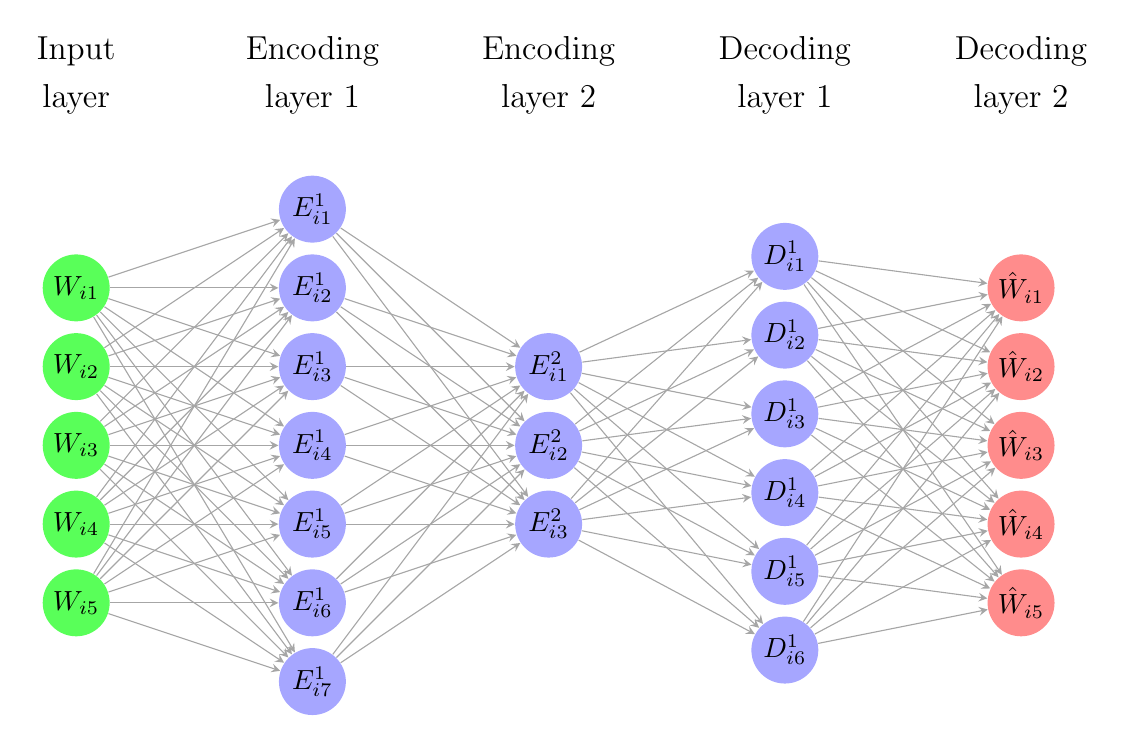
\begin{tikzpicture}[
    >=stealth,
    inputnode/.style={circle, fill=green!65, minimum size=8.5mm, inner sep=0pt},
    hiddennode/.style={circle, fill=blue!35, minimum size=8.5mm, inner sep=0pt},
    outputnode/.style={circle, fill=red!45, minimum size=8.5mm, inner sep=0pt},
    conn/.style={gray!70,->,thin}
]

% Layer titles
\node[font=\large] at (0,5.8) {Input};
\node[font=\large] at (0,5.2) {layer};

\node[font=\large] at (3,5.8) {Encoding};
\node[font=\large] at (3,5.2) {layer 1};

\node[font=\large] at (6,5.8) {Encoding};
\node[font=\large] at (6,5.2) {layer 2};

\node[font=\large] at (9,5.8) {Decoding};
\node[font=\large] at (9,5.2) {layer 1};

\node[font=\large] at (12,5.8) {Decoding};
\node[font=\large] at (12,5.2) {layer 2};

% Input layer: 5 nodes
\foreach \i/\y in {1/2.8,2/1.8,3/0.8,4/-0.2,5/-1.2}
    \node[inputnode] (I\i) at (0,\y) {$W_{i\i}$};

% Encoding layer 1: 7 nodes
\foreach \j/\y in {1/3.8,2/2.8,3/1.8,4/0.8,5/-0.2,6/-1.2,7/-2.2}
    \node[hiddennode] (Eone\j) at (3,\y) {$E^{1}_{i\j}$};

% Encoding layer 2: 3 nodes
\foreach \j/\y in {1/1.8,2/0.8,3/-0.2}
    \node[hiddennode] (Etwo\j) at (6,\y) {$E^{2}_{i\j}$};

% Decoding layer 1: 6 nodes
\foreach \j/\y in {1/3.2,2/2.2,3/1.2,4/0.2,5/-0.8,6/-1.8}
    \node[hiddennode] (Done\j) at (9,\y) {$D^{1}_{i\j}$};

% Output layer: 5 nodes
\foreach \i/\y in {1/2.8,2/1.8,3/0.8,4/-0.2,5/-1.2}
    \node[outputnode] (O\i) at (12,\y) {$\hat W_{i\i}$};

% Connections: input -> encoding 1
\foreach \i in {1,...,5}
    \foreach \j in {1,...,7}
        \draw[conn] (I\i) -- (Eone\j);

% Connections: encoding 1 -> encoding 2
\foreach \i in {1,...,7}
    \foreach \j in {1,...,3}
        \draw[conn] (Eone\i) -- (Etwo\j);

% Connections: encoding 2 -> decoding 1
\foreach \i in {1,...,3}
    \foreach \j in {1,...,6}
        \draw[conn] (Etwo\i) -- (Done\j);

% Connections: decoding 1 -> output
\foreach \i in {1,...,6}
    \foreach \j in {1,...,5}
        \draw[conn] (Done\i) -- (O\j);

\end{tikzpicture}
\end{document}